\subsection{Direct Detection}
After executing the flavour processes where the NP states had the role of mediators, we now turn towards the phenomenological aspects of DM itself.
We begin with direct detection (DD) or nucleon ($N$) scattering where a DM particle scatters off a parton (quark or gluon) of a nucleon. 
\\ \\ \textit{Effective Lagrangian}\\
This can happen
due to a spin independent (SI) or spin dependent (SD) interaction \eqref{eq_th.sigma.dd} which are described by an effective Lagrangian \cite{1104.0228}
\begin{align}
 \mathcal{L}^\text{eff} = \sum\limits_{q} \mathcal{L}^\text{eff}_q + \mathcal{L}^\text{eff}_g.
\end{align}
We use $q$ for the light quarks $u$, $d$, $s$ and $Q$ for heavier $c$, $b$, $t$. From \eqref{eq_fierzSPtoVA} we see that from our chiral model, 
we only get effective interactions with quarks like $\bar \chi\gamma^\mu\chi \bar q\gamma_\mu q$ and $\bar \chi\gamma^\mu\gamma_5 \bar q\gamma_\mu \gamma_5 q$
as six dimensional operators. The former vanishes for Majorana DM and the latter is SD which will not give stronger constraints than the following SI
interactions but the resulting SD cross section can be evaluated with the expressions also given in \cite{1104.0228} for the leading processes to be of
order $\mathcal{O}(10^{-44})$ cm$^2$ while the upper limits obtained by IceCube \cite{1212.4097} yield $\mathcal{O}(10^{-40})$ cm$^2$ for 
a 100 GeV'ish DM particle.
So we neglect them. A possibly occuring scalar operator $f_q m_q\bar \chi \chi \bar q q$ also vanishes for tree level processes in our chiral model
but is enabled at loop level. Therefore the first contributing
SI operators coming from quark interactions are eight dimensional, namely those depending on twist-2 operators. They are the traceless parts of the
quark energy momentum tensor and arise from the matrix element of a quark current product expressed in local operators \cite{MDSchwartz}. The twist of 
an operator is definded as the difference between its mass dimension and its spin. So much for the quark interaction. Since our DM particle shall be an 
$SU(3)_C$-singlet, it does not couple directly to gluons $g$ but scalarlike at one-loop level through the heavy quarks. There is also a twist-2 
operator for the gluon but its coefficient will be suppressed by $\alpha_s$ so we will not consider it further. So at least for our $SU(2)_L$ singlet
DM particle which does not interact with the $W$ bosons, the leading SI Lagrangian is
%For both DM $SU(2)_L$-representations, the singlet and the triplet, the leading SI operators are
\begin{align}
 \mathcal{L}^\text{eff} =&\, \frac{g_q^{(1)}}{m_\chi} \bar \chi\ti \partial_\mu \gamma_\nu O_q^{\mu\nu} + \frac{g_q^{(2)}}{m^2_\chi} \bar \chi(\ti \partial_\mu) (\ti\partial_\nu) O_q^{\mu\nu} \\
 \nonumber
 &+ f_G \bar \chi \chi G^a_{\mu\nu} G^{a\mu\mu}.
\end{align}
The twist-2 operator for the quark is
\begin{align}
 O_q^{\mu\nu} = \frac12 \bar q \ti \left(D^\mu \gamma^\nu + D^\nu \gamma^\mu - \frac12 g^{\mu\nu} \slashed{D}\right) q
\end{align}
with $D_\mu$ as the covariant derivative for $SU(3)_C$ and the three coefficients of mass dimension $-3$ $g_q^{(1)}$, $g_q^{(2)}$ and $f_G$ enter 
the form factor $f_N$ in \eqref{eq_th.sigma.dd} as
\begin{align}
 \frac{f_N}{m_N} = \sum\limits_{q,c,b} \frac34 \left(q(2)+\bar q(2)\right) \left(g_q^{(1)} + g_q^{(2)}\right) - \frac{8\pi}{9\alpha_s}f_{TG}f_G
 \label{eq_ddformfactorA}
\end{align}
where the matrix elements of the effective operators are expressed with the nucleon mass $m_N$ as \cite{1007.2601}
\begin{subequations}
\begin{align}
 \langle N(p)| O_q^{\mu\nu} | N(p)\rangle =& \frac{1}{m_N}\left(p^\mu p^\nu - \frac14 m_N^2 g^{\mu\nu}\right) \left(q(2) + \bar q(2)\right),\\
 f_{TG} :=& 1- \sum\limits_q f_{Tq},\\
 f_{Tq} :=& \langle N|m_n \bar qq |N\rangle /m_N.
\end{align}
\end{subequations}
The quantities $q(2)$ and $\bar q(2)$ are the second moments \cite{0811.1779} of the parton distribution function (PDF) of quark $q(x)$ or antiquark 
$\bar q(x)$, respectively, in the nucleon $q(2)+\bar q(2) = \int_0^1 \dx x\, x^2 \left[q(x) + \bar q(x)\right]$. The values used for the numerical
calculation are listed in tabular \ref{tab_parton}.
\begin{table}[b]
 \begin{tabular}{c|ccccc}
   & $u$ & $d$ & $s$ & $c$ &$b$ \\
   \hline
  $q(2)$ & 0.22 & 0.11 & 0.026 & 0.019 & 0.012\\
  $\bar q(2)$ & 0.034 & 0.036 & 0.026 & 0.019 & 0.012\\
  $f_{Tq}$ & 0.020& 0.026 & 0.134 (1209.3641)\\
 \end{tabular}
\caption{Second moments $q(2)$, $\bar q(2)$ of the quark PDFs evaluated at $\mu=m_Z$ and taken from \cite{0201195} and scalar matrix elements $f_{Tq}$ of 
the light quarks for the 
proton each. For the neutron $u(2)$ and $d(2)$ just swap and $f_{Tu}$ and $f_{Td}$ differ slightly \cite{9506380}. All other quantities are the same. }
\label{tab_parton}
\end{table}
\noindent The evaluation of $f_G$ is factorised in a ``short distance'' (SD, not to confuse with spin dependency) and a ``long distance'' (LD) 
contribution
\begin{align}
 f_G|_q = f_G|^\text{SD}_q + f_G|^\text{LD}_q. 
\end{align}
The former (latter) represents a scale of heavy (light) particles as the colored scalar mediator (quarks). While we need to calculate the full
loop process e.g. in figure \ref{pic_ddsinglet} for the SD, the LD with $Q$ can be thought of a triangle diagram where $\Phi_q$ integrated 
out i.e. there arises a four fermion operator $f_Q m_Q \bar \chi \bar Q Q$. The triangle loop calculation yields in the heavy scalar mass limit 
\begin{align}
 f_G|_Q^\text{LD} = -\frac{\alpha_s}{12\pi} c_Q f_Q,
 \label{eq_longdistance}
\end{align}
with $c_Q = 1+11\alpha_s(m_Q)/4\pi$ coming from large QCD corrections \cite{Djouadi}, $c_c=1.32$, $c_b = 1.19$, $c_t = 1$.
When considering the light quarks $q$ in the LD term, they have a vanishing contribution since the respective operator goes with the quark mass
which is each smaller than $\Lambda_\text{QCD} = \mathcal{O}(100)$ MeV and their propagators are entirely determined by confinement dynamics. Thus,
we do not have to take them into account. The explicit formula for the operator coefficients \eqref{eq_ddformfactorA} for the singlet case 
will be given now.
\\ \\ \textit{Singlet Dark Matter}\\
\begin{figure}[t]
 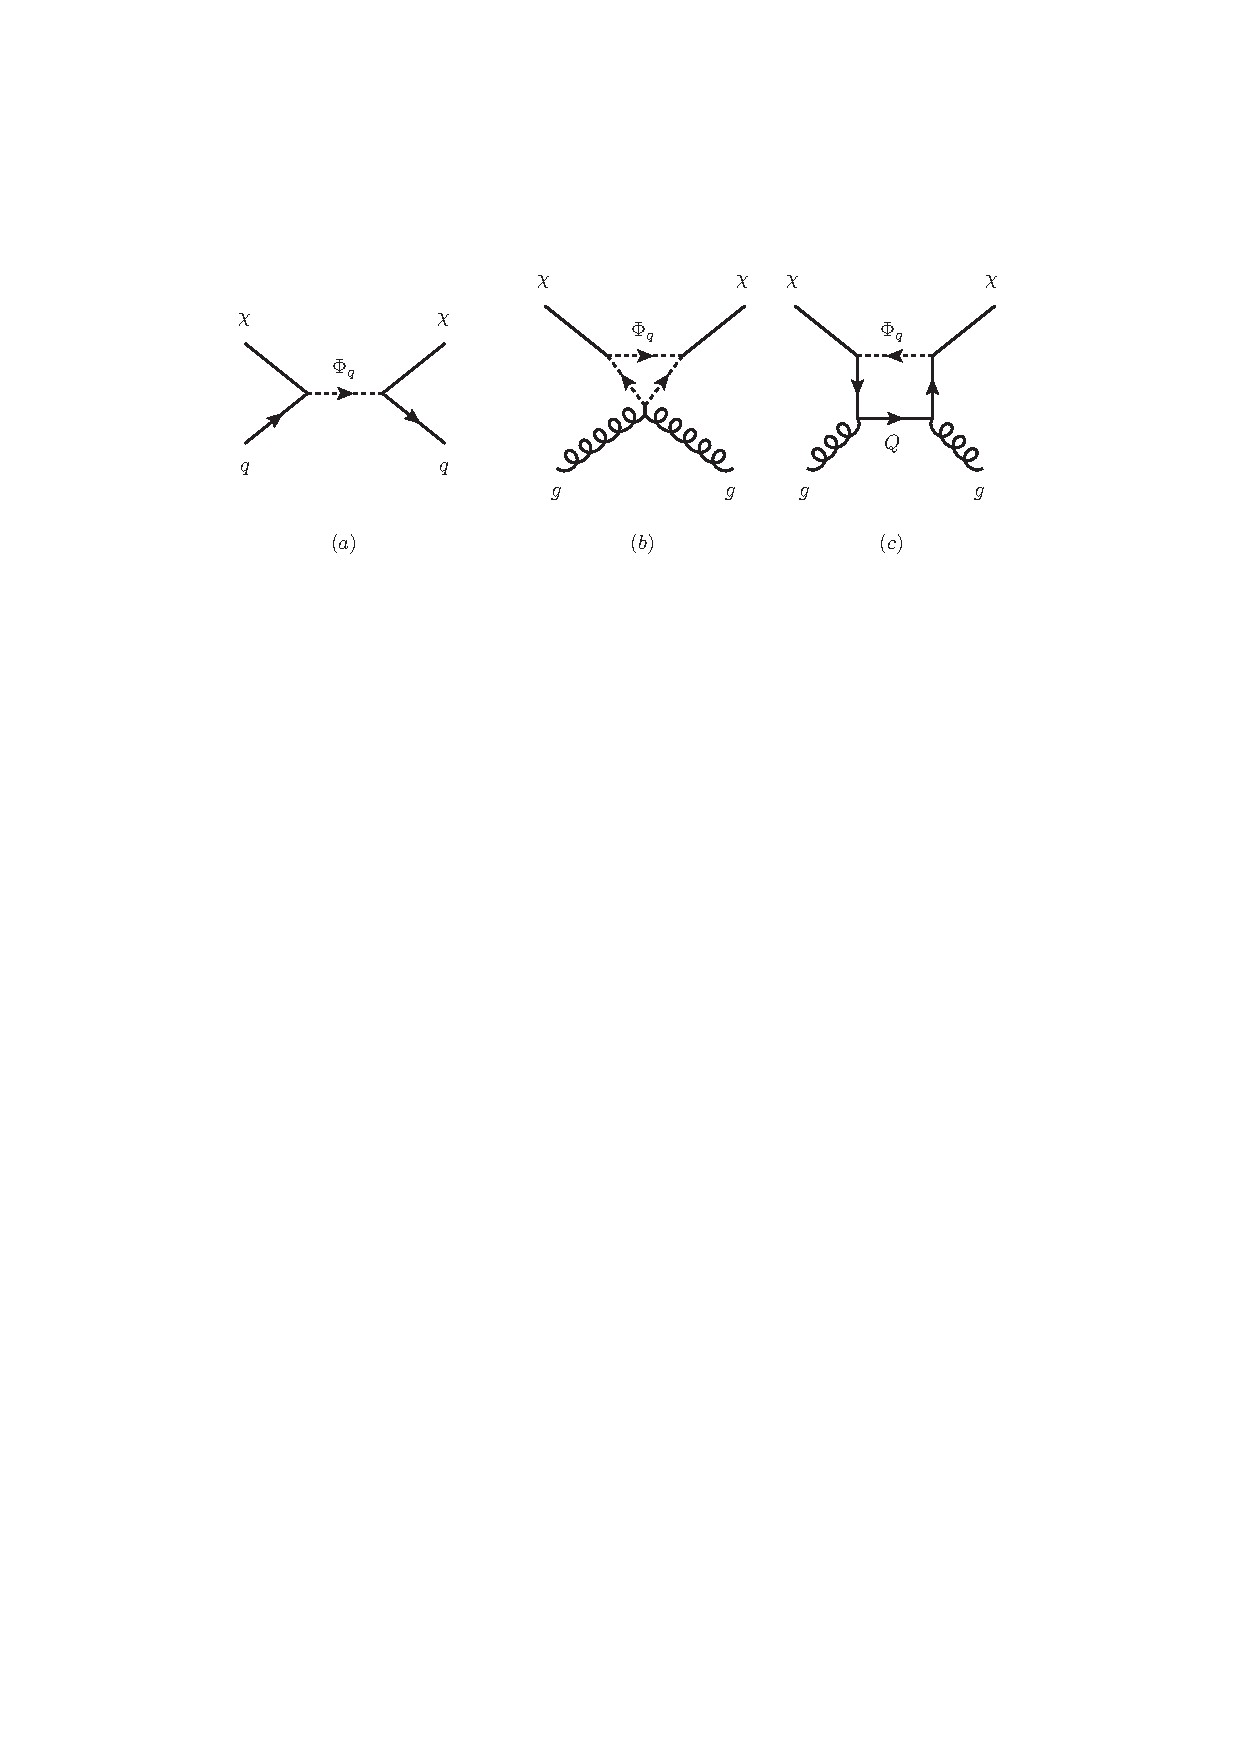
\includegraphics[width=1\textwidth]{../pics/ddsinglet.pdf}
 \caption{DM scatters off quarks at tree level and off gluons at one loop order.}
 \label{pic_ddsinglet}
\end{figure}
The $\chi$-q interaction is visualised in figure \ref{pic_ddsinglet}(a) and is easily computed in this s-channel process. After integrating out the 
scalar and in the massless quark limit the coefficients are
\begin{align}
 g_q^{(1)} = \frac{|g_q|^2 }{4} \frac{m_\chi}{\left(m_\chi^2 - M_{\Phi_q}^2\right)^2},
 g_q^{(2)} = 0.
\end{align}
For degenerate DM and messenger mass, there would also be a term with the decay width $\Gamma$ of the messenger in the denominator to avoid the 
divergence, but we assume anyway the scalar to be way heavier than the fermion. %(TODO why is g2q zero). 
The effective gluonic coupling in the 
singlet case will be derived from one loop processes (fig. \ref{pic_ddsinglet}b, c) 
% \begin{figure}[t]
%  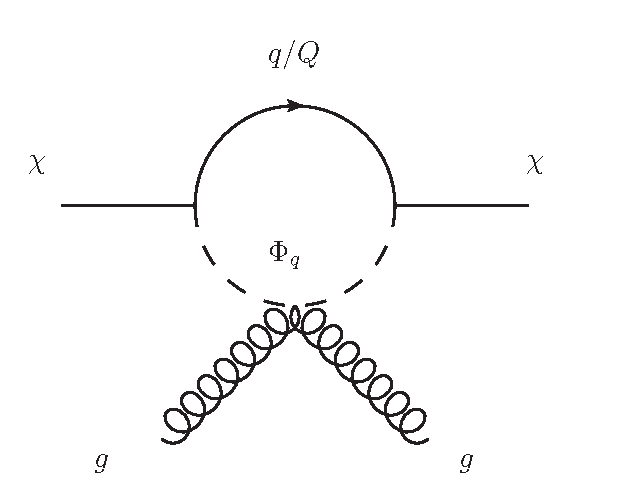
\includegraphics[width=0.5\textwidth]{../pics/phigluon.eps}
%  \caption{One loop diagrams contributing to the effective gluonic coupling.}
%  \label{pic_ddGluonA}
% \end{figure}
for which we take the Fock-Schwinger gauge for the gluon
field $x^\mu G^a_\mu = 0$. Effectively we can express $f_G = \Gamma_\chi(p)/2|_{GG}$ as a two-point function... The SD and LD terms thereof are
\begin{align}
 f_G^\text{SD}|_q = \frac{\alpha_s}{32\pi} m_\chi f^s,\\
 f_G^\text{LD}|_q = \frac{\alpha_s}{32\pi} m_\chi f^l.
\end{align}
with the loop functions $f$ in the zero quark mass limit
\begin{align}
 f^s \stackrel{m_q=0}{=} - \frac{1}{6M_{\Phi_q}^2\left(M_{\Phi_q}^2-m_\chi^2\right)} \stackrel{M_{\Phi_q}\gg m_\chi}{=} -\frac{1}{6M_{\Phi_q}^4},\\
 f^l \stackrel{m_q=0}{=} - \frac{1}{6\left(M_{\Phi_q}^2-m_\chi^2\right)^2}  \stackrel{M_{\Phi_q}\gg m_\chi}{=} -\frac{1}{6M_{\Phi_q}^4}.
\end{align}
Gathering up the SD and LD terms, the scalar $\chi$-g interaction coefficient is
\begin{align}
 f_G = -\frac{\alpha_s}{96\pi} \frac{m_\chi}{M_{\Phi_q}^4} \sum\limits_{\text{all}} |g^q|^2
\end{align}
and the full form factor \eqref{eq_ddformfactorA} can be written in these limits as
\begin{align}
 \frac{f_N}{m_N} = \frac{m_\chi}{M_{\Phi_q}^4} \sum\limits_\text{all} \left|g^q\right|^2 \left[\frac{f_{TG}}{108} + \frac{3}{12}\left(q(2) + \bar q(2)\right)\right].
\end{align}
Even though every quark participates, we go on only with the bottom quark and the top which appears only in the gluon term because they deliver the
largest part to the form factor. The SI cross section \eqref{eq_th.sigma.dd} can now be written as
\begin{align}
 \sigma_\text{SI} = \frac{4}{\pi}\mu_N^2 \left| f_N \right| ^2 \approx 2.33\cdot 10^{-4} \mu_N^2 \cdot |g^q_3|^4 \frac{m_\chi^2 m_N^2}{M_{\Phi_q}^8}
 \label{eq_sigmaDDA}
\end{align}
For a 100 GeV'ish DM fermion and a 1 TeV'ish messenger, we would have an SI $\chi-N$ cross section of $\mathcal{O}(10^{-51})$ cm$^2$ which is far 
below current bounds. Hence we do not expect exclusion from direct detection for our singlet case and so we look at the triplet case.
\\ \\ \textit{Triplet Dark Matter}\\
\begin{figure}[t]
 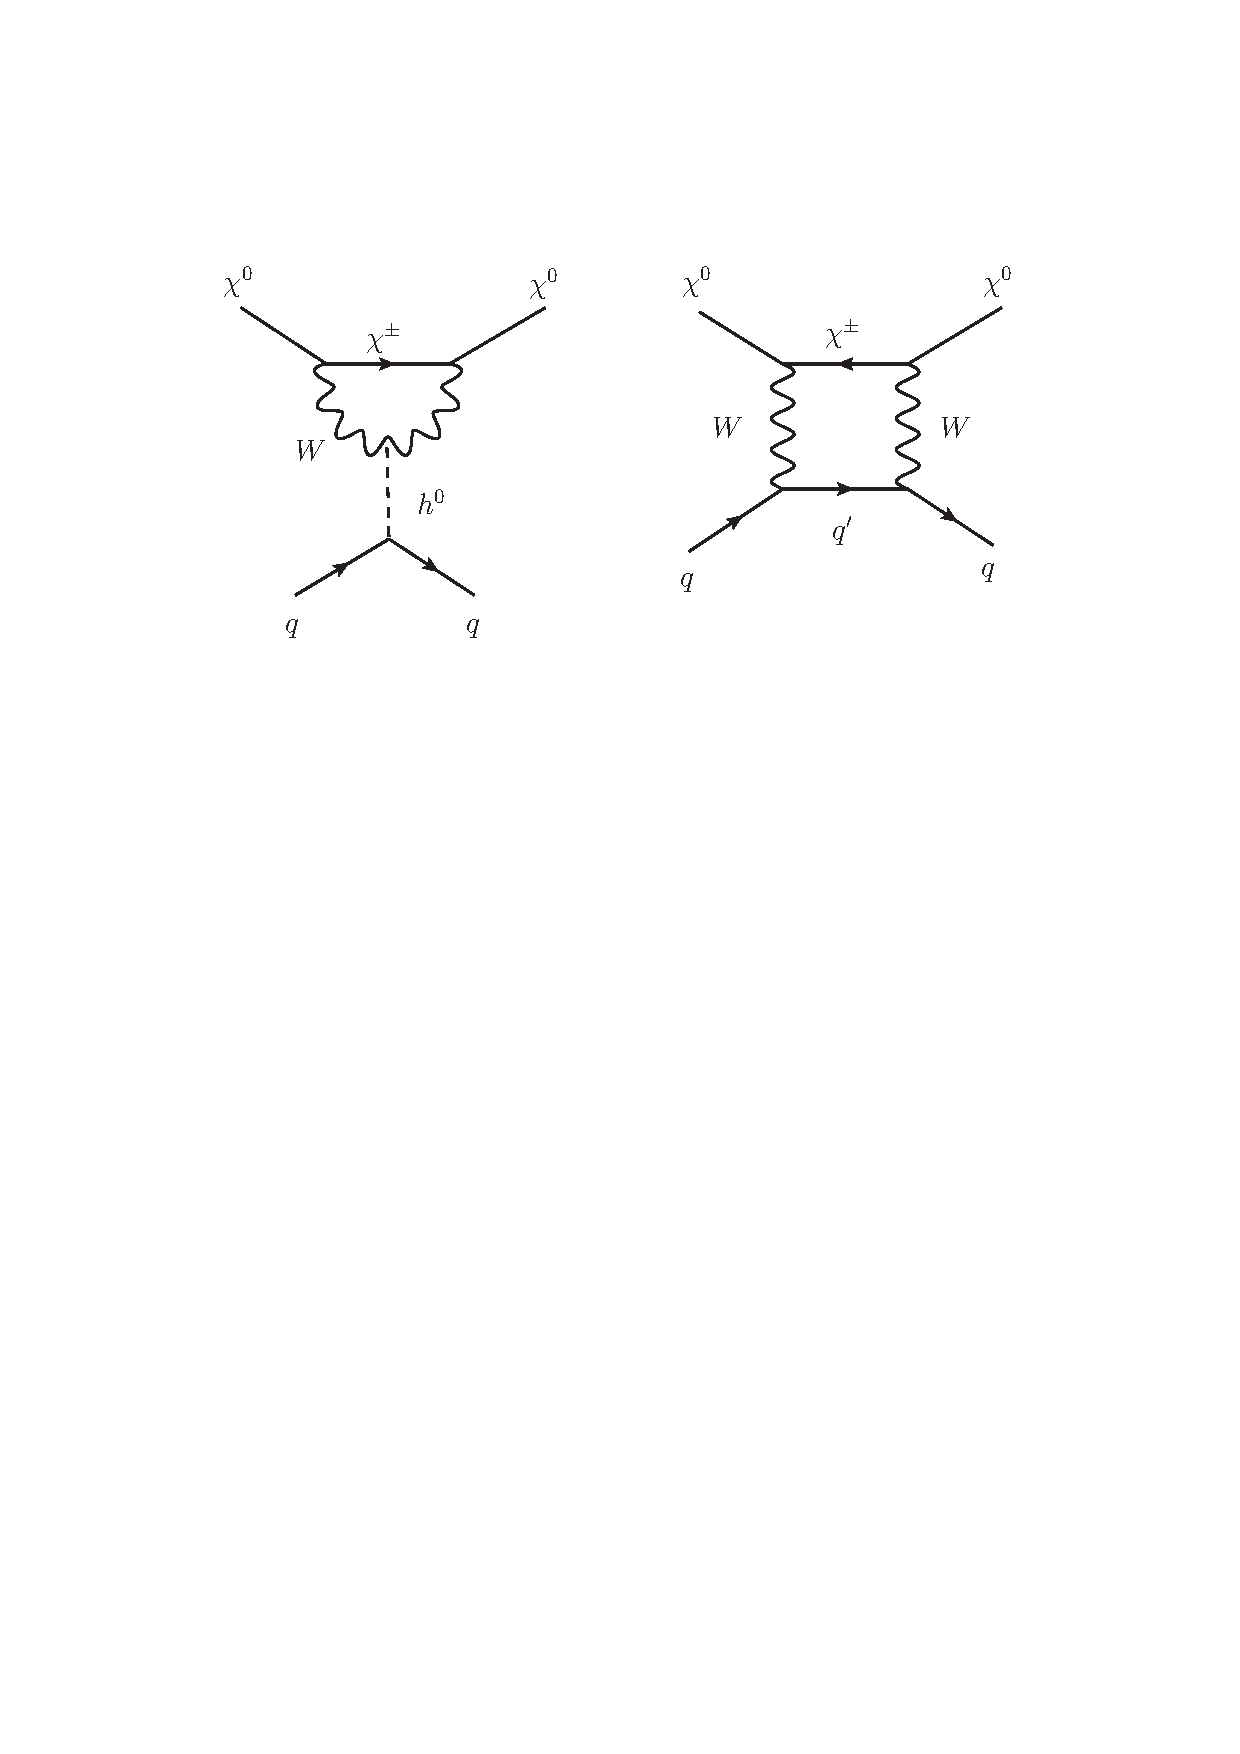
\includegraphics[width=0.7\textwidth]{../pics/wloops.pdf}
 \caption{One loop processes for the effective $\chi^0-N$ coupling. Penguins with a photon or a $Z$-boson turn out to vanish(\cite{1104.0228}).}
 \label{pic_wloop}
\end{figure}
The main difference between the $SU(2)_L$ singlet and the triplet is the interaction with the weak boson $W$. While the singlet does not couple to
it directly, the $W$ couples to two particle states within the triplet whose electric charges differ by one. Just to recall, in neither case the 
DM particle carries hypercharge, so that the respective neutral component does not couple to the $Z$ boson. The interative Lagrangian for the $W$ 
boson is 
\begin{align}
 \mathcal{L} = \frac{g_2}{\sqrt{2}} \left[\bar \chi^0 \gamma^\mu \chi^- W^+_\mu + \bar \chi^0 \gamma^\mu \chi^+W^-_\mu\right] +\, \text{h.c.}
\end{align}
Since the cross section in the singlet case \eqref{eq_sigmaDDA} was driven by the large scalar mass we can take advantage of the possible processes
for direct detection which do not involve the scalar \cite{1004.4090}. In fact, the form factor is dominated by one loop processes with a $W$ for an interaction with
quarks (see fig. \ref{pic_wloop}) and two loop processes for gluonic scattering (see fig. \ref{pic_2loopgluon}).
\begin{figure}[t]
 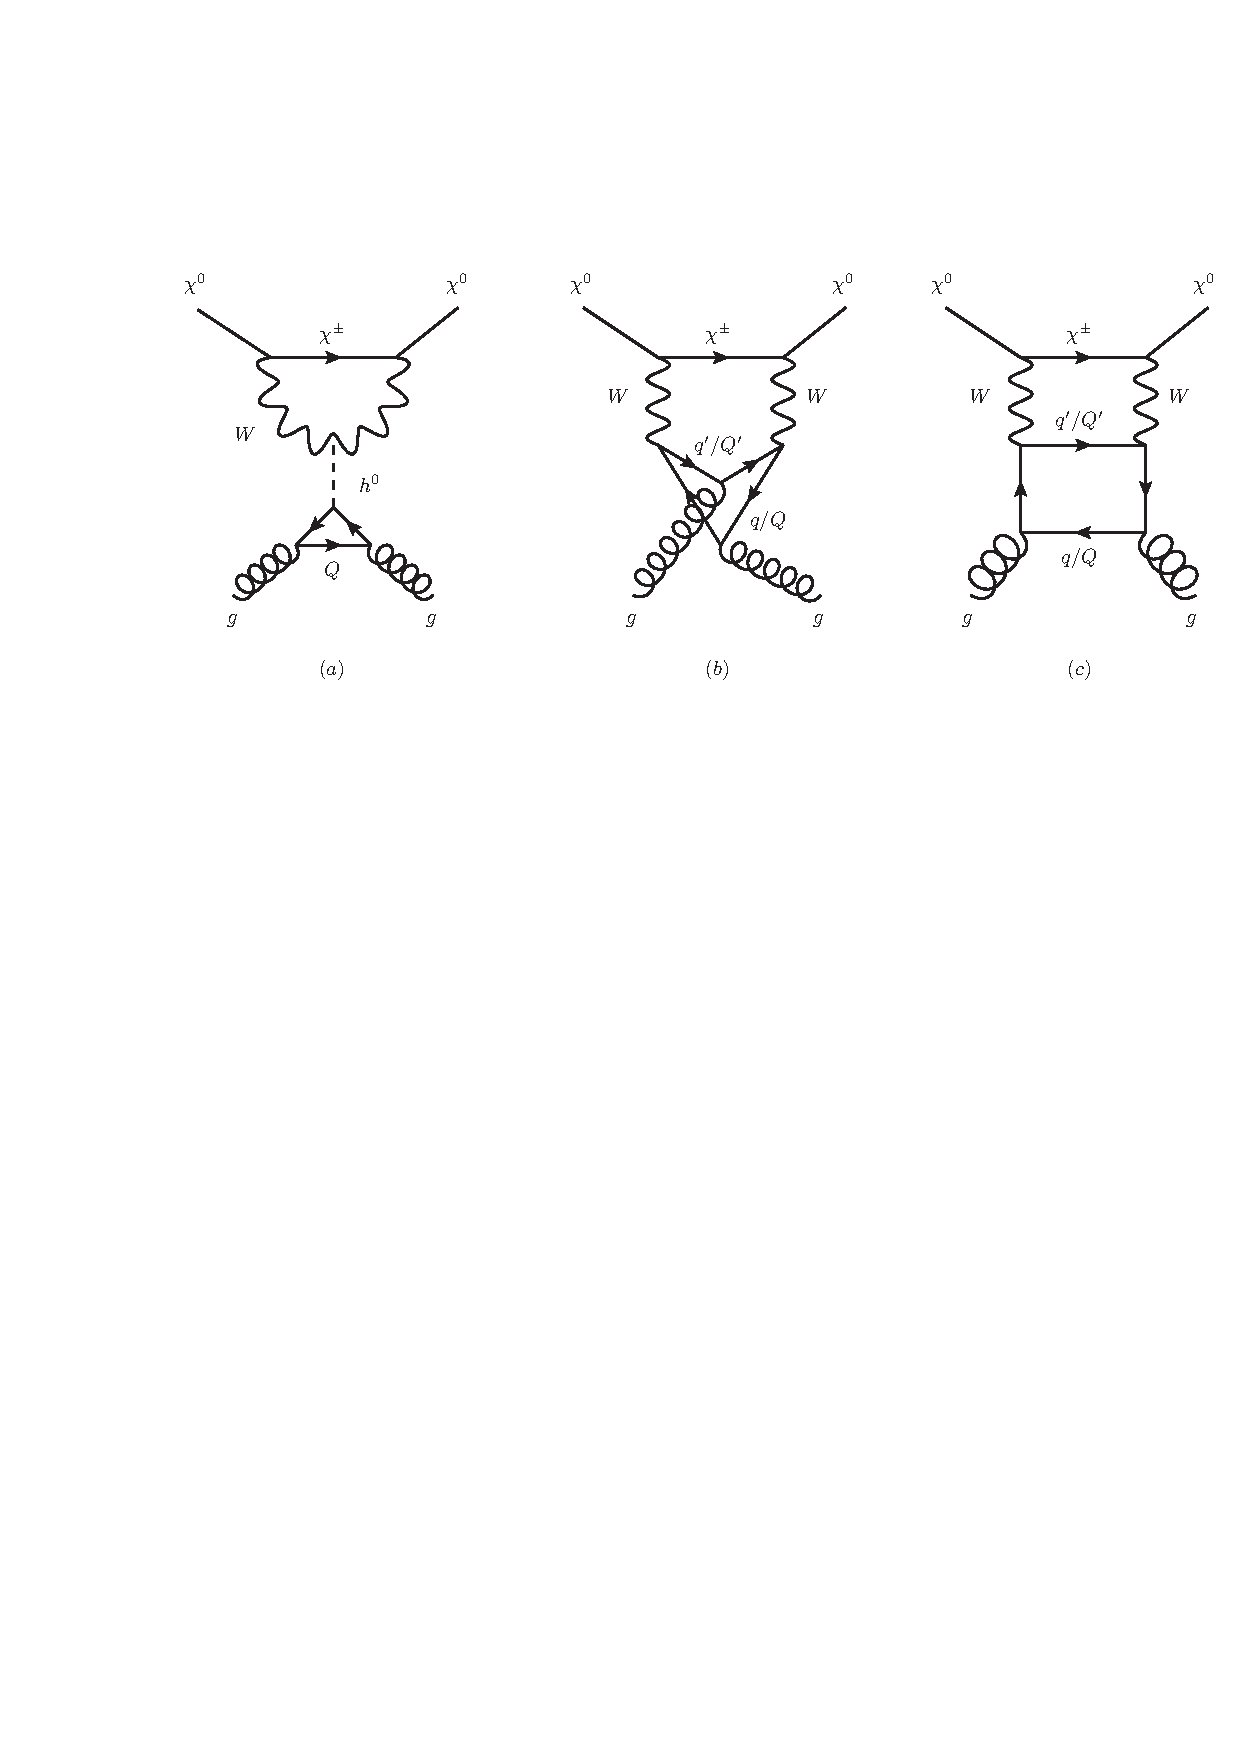
\includegraphics[width=1\textwidth]{../pics/gluon2loopB.pdf}
 \caption{Two loop diagrams contributing to the effective gluonic coupling.}
 \label{pic_2loopgluon}
\end{figure}
For the effective $\chi^0-q$-coupling we get
\begin{align}
 f_q =& \frac{\alpha_2^2}{4m_W m_{h}^2} g_H(w)\\
 g^{(1)}_q =& \frac{\alpha_2^2}{m_W^3}g_{T1}(w)\\
 g^{(2)}_q =&\frac{\alpha_2^2}{m_W^3}g_{T2}(w) 
\end{align}
where $f_q$ gets its contributions from $h^0$ exchange and the $W$-box leads to $g^{(i)}_q$. Also $m_W$ and $m_h$ stand for the $W$-mass and the 
$h^0$-mass, respectively.\\
\noindent Concerning the gluonic coupling, we have three dominating two loop processes, one via Higgs exchange (fig. \ref{pic_2loopgluon}a) and two
$W$-boxes (fig. \ref{pic_2loopgluon}b, c). The first one is evaluated easily by comparing it to the effective quark coupling from figure \ref{pic_wloop}a
by exchanging the light scattered quarks with heavy quarks and contributes hence to the LD interaction \eqref{eq_longdistance}. The calculation of 
the other two diagrams is a little cumbersome since the loops have to be calculated explicitly with the additional treatment of the vacuum polarisation
tensor of the $W$ \cite{1007.2601}. In the end we have for the effective $\chi^0-g$-coupling
\begin{align}
 f_G = \frac{\alpha_s\alpha_2^2}{4\pi m_W}\left(-\sum\limits_Q c_Q \frac{1}{3m_{h^0}^2} g_H(w) + \frac{1}{m_W^2} g_{W}(w,t) \right)
\end{align}
with $w=\sfrac{m_W^2}{m_\chi^2}$ and $t=\sfrac{m_t^2}{m_\chi^2}$ ($m_t$ is the top mass).
So with the additional scalar $\chi^0$-$q$ coupling giving a contribution to the form factor as $\sum_qf_{Tq}f_q$, the result is
\begin{align}
 \frac{f_N}{m_N} =& \frac{\alpha_2^2}{m_W^3}\left(\sum\limits_{q,c,b} \frac34 \left(q(2)+\bar q(2)\right) \left(g_{T1}(w) + g_{T2}(w)\right) + \frac29g_W(w,t)\right) \\
 \nonumber
 &+ \frac{\alpha_2^2}{m_W m_h^2}g_H(w) \left(\frac14 \sum\limits_q f_{Tq} - \frac{2}{27}\sum\limits_Q c_Q \right)
\end{align}
The SI cross section for the triplet can now be calculated easily but the loop functions just mentioned have no common dependencies on the DM mass
so that no compact expression for SI cross section can be presented. As stated in the beginning of this paragraph, the cross section only depends
on $m_\chi$. The mass difference of the charged triplet components to the neutral one is assumed to be negligable compared to the mass scale itself,
so they do not enter explicitly. 

% \begin{align}
%  \sigma_\text{SI} = \frac{4}{\pi}\mu_N^2 \left| f_N \right| ^2 \approx 4.57\cdot 10^{-18} \mu_N^2 \cdot \left(0.51 \left(g_{T1}+g_{T2}\right) + \frac29 g_W - 0.02 g_H\right)
%  \label{eq_sigmaDDB}
% \end{align}
% with the masses in GeV. Unlike \eqref{eq_sigmaDDA} the cross section for the triplet case only depends on the DM mass which makes it generally very
% interesting in constraining such models. 











